%!TEX ROOT=radek-novotny-bp-2017.tex
\chapter{Praktická část}
\label{4-prakticka-cast} Následující kapitola pojednává o výsledku
celé této práce, zásuvném modulu Soil Erosion pro QGIS, a to zejména o
zvolených technických řešeních. Informace o~pluginu z pohledu
%%% ML: uvest link na prilohu (\ref{})
uživatele shrnuje manuál nacházející se v příloze.
\section{Vývoj} Při vývoji pluginu bylo čerpáno z literatury o
programu QGIS\cite{masteringQgis} a programovacím jazyce
Python\cite{learningPython}\cite{diveIntoPython}, ale také využito
internetu a zkušeností široké základny vývojářů
%%% ML: stackexchange je mozna prilis obecny, lepsi ML
%%% https://lists.osgeo.org/mailman/listinfo/qgis-user
QGIS\cite{stackexchange}. Celý vývoj probíhal v angličtině s využitím
%%% ML: davejte si pozor na dlouha souveti. V textu je jich
%%% hodne. Exemplar nize jsem rozdelil.
webové služby GitHub (kap.~\ref{github}), jež podporuje verzovací
nástroj Git. Celá práce je tedy, kromě přiloženého CD, dostupná právě
i z GitHub repositáře\cite{mujgithub}.
\subsection{Kostra} Pomocí zásuvného modulu Plugin Builder, který je
zařazen do oficiálního repositáře QGIS~(kap.~\ref{qgis}), byl vytvořen
adresář se základní kostrou pluginu obsahující soubory se základním
grafickým uživatelským rozhraním (GUI), zdrojovým kódem a informacemi
o zásuvném modulu.
\subsection{Grafické uživatelské rozhraní} Na tuto základní kostru
bylo navázáno vytvořením GUI v programu
Qt~Designer (kap.~\ref{qt}). Modul je tvořen jedním oknem z třídy
\texttt{QDockWidget}, jež umožňuje ukotvení pluginu do rozhraní
programu QGIS. V tomto okně je vnořen objekt třídy \texttt{QTabWidget}
rozdělující GUI na pět záložek – EUC pro definici vrstvy obsahující
erozně uzavřené celky a dále LS, K, C a RP, které tematicky odpovídají
faktorům rovnice USLE počítaným ze zadaných vstupů.

Definování vstupů v jednotlivých záložkách probíhá pomocí
rozbalovacího seznamu z třídy \texttt{QgsMapLayerComboBox}, který
obsahuje vrstvy načtené v QGIS. Pro tento seznam bylo nastaveno
omezení typu vrstvy dle požadavků dalšího výpočtu.  Druhou možností
vstupu vrstvy je tlačítko třídy \texttt{QPushButton}, které načítá do
QGIS novou vrstvu znovu s omezením na její typ. Poslední typ vstupu se
%%% ML: ve vete 2x "pomoci"
nachází v záložce RP, jedná se o vstup pomocí pole třídy
\texttt{QLineEdit} pomocí zapsání číselné hodnoty.

V modulu jsou také další tři tlačítka z třídy \texttt{QPushButton}. V
záložkách K a C jsou to tlačítka pro výpočet jednotlivých faktorů ve
zvolené vstupní vrstvě a pod záložkami se nachází tlačítko spouštějící
výpočet erozního modelu. Všechny objekty modulu se také přizpůsobují
zvolené šířce okna.
\subsection{Zdrojový kód} Zdrojový kód byl psán v jazyce Python
2.7~(kap.~\ref{python}) ve vývojovém prostředí PyCharm, vyvinutém
českou společností JetBrains. Dále byl pro testování změn v~kódu
použit Plugin Reloader, který je stejně jako Plugin Builder součástí
oficiálního repositáře QGIS.
\subsection{Lokalizace} Jelikož byl celý zásuvný modul vyvíjen v
angličtině, došlo v poslední fázi k jeho překladu a lokalizaci do
češtiny. K tomu byl využit program Qt Linguist.

\section{Popis struktury kódu} Strukturu kódu lze rozdělit na dvě
části – tělo modulu a knihovnu \textit{pyerosion}.
%%% ML: nekde o tridy ale spise o "modulu" (python soubory)
\subsection{Knihovna pyerosion} Tato knihovna obsahuje třídu
\texttt{erosionbase.py} vycházející z projektu QGIS Erosion
plugin\cite{erosiongithub} a vytvořené třídy \texttt{erosionusle.py} a
\texttt{read\_csv.py}.
\subsubsection{Třída ErosionBase} Tato třída v původní formátu
sloužila ke spuštění programu GRASS GIS 7~(kap.~\ref{grassgis}) a
nastavení výpočetního prostředí, tedy lokace a mapsetu. Dále byla
využita pro import dat do tohoto programu. Tyto funkce byly využity
při volání nástrojů GRASS GIS ze zásuvného modulu. Nově byla vytvořena
funkce pro export dat, která je uplatněna při exportu výsledků z GRASS
GIS zpět do QGIS.
\subsubsection{Třída ErosionUSLE} Ve třídě \texttt{ErosionUSLE} dědící
z \texttt{ErosionBase} probíhá veškerý výpočet odehrávající se v
prostředí GRASS GIS. K tomu je využito příkaz \texttt{run\_command} z
Python knihovny systému GRASS \texttt{grass.script.core}. Podrobný
%%% ML: doplnit
postup je popsán dále v $-----------$

\subsubsection{Třída ReadCSV} Třída \texttt{ReadCSV} slouží ke čtení
CSV (comma-separated values) souborů, ve kterých jsou uloženy hodnoty
K faktoru pro jednotlivé HPJ a C faktoru pro osevní postupy. Tyto
soubory jsou uloženy v adresáři \texttt{code\_tables}.

\subsection{Tělo zásuvného modulu} Tělo zásuvného modulu je tvořeno
souborem \texttt{soil\_erosion\_dockwidget.py} s hlavní třídou
\texttt{SoilErosionDockWidget} propojenou s grafickým uživatelským
rozhraním umístěným v souboru
\texttt{soil\_erosion\_dockwidget\_base.ui}. V této třídě jsou
%%% ML: objekty -> asi lepe "widgety"
definovány funkce pro jednotlivé objekty GUI, import dat a výpočetní
část probíhající v QGIS. Jsou zde také definovány chybové hlášení, jež
jsou vypsány při nesprávném vstupu či chybě ve výpočtu. V druhé třídě
%%% ML: souboru -> asi lepe "modulu"
tohoto souboru \texttt{ComputeThread} dochází ke spuštění výpočtu v
systému GRASS GIS, který probíhá v samostatném výpočetním vlákně a
neovlivňuje další funkce QGIS. Během výpočtu jsou pomocí signálů
přenášeny zprávy o stavu výpočtu na informační panel QGIS.

\paragraph{Dalšími součástmi těla pluginu jsou soubory:}
\begin{itemize}
	\item \texttt{init.py} - Sloužící k základní inicializaci
pluginu.
	\item \texttt{soil\_erosion.py} – Sloužící k zařazení pluginu
do prostředí QGIS, jeho spuštění a ukončení.
	\item \texttt{plugin\_upload.py} – Soubor pro nahrání modulu
do QGIS repositáře zásuvných modulů.
	\item \texttt{metadata.txt} – Textový soubor obsahující údaje
o pluginu.
	\item \texttt{Makefile} – Slouží ke zkompilování resources.py
nebo dokumentace.
	\item \texttt{resources.py} – Zkompilovaný soubor
resources.qrc, poskytuje informace o ikoně pluginu.
	\item \texttt{Icon.png} – Ikona pluginu.
\end{itemize}
\newpage
\subsection{Schéma výpočtu} Zde je zobrazeno schéma výpočtu barevně
odlišující část probíhající v QGIS od části probíhající v systému
GRASS GIS. Postup výpočtu částečně vychází z
\textit{Gismentors}\cite{gismentors}. Jednotlivé kroky výpočtu jsou
rozebrány dále.
\begin{figure}[H]
\centering 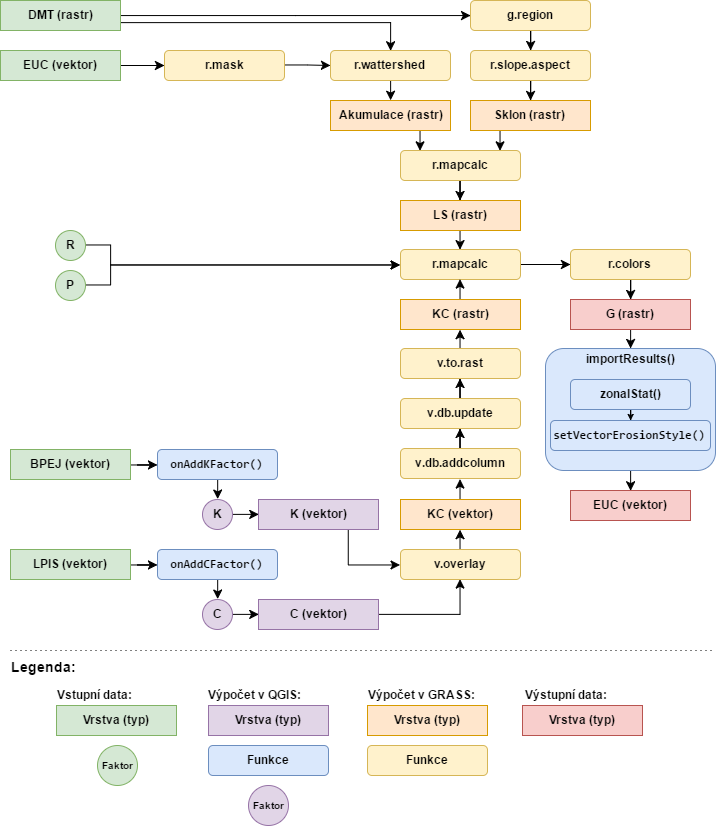
\includegraphics[scale=0.6]{./pictures/diagram.png}
      \caption[Diagram výpočtu] {Diagram výpočtu, zdroj: autor}
      \label{diagram}
\end{figure}
\newpage
\subsection{Popis výpočtu v GRASS GIS a použitých modulů} Tato sekce
popisuje funkce, vstupy a výstupy použitých modulů, tj. nástrojů systému GRASS GIS.
\begin{enumerate}
	\item \texttt{g.region} – Nastavení výpočetního regionu.
	\item \texttt{r.slope.aspect} – Výpočet sklonu na základě
          rastru DMT.
          %%% ML: maska se nastavuje aktualne z EUC
	\item \texttt{r.mask} – Nastavení masky podle zájmového území,
tedy rastru DMT.
	\item \texttt{r.watershed} – Výpočet akumulace odtoku na
základě rastru DMT. (Tato funkce byla upřednostněna před funkcí
\texttt{r.terraflow} na základě \textit{Metodiky GIS pro navrhování
TPEO}\cite{Dostal2014}.)
	\item \texttt{r.mapcalc} – Pomocí mapové algebry vypočítán
faktor LS na základě sklonu, akumulace a rozlišení rastrů dle rovnice
\ref{ls_faktor}.
	\item \texttt{v.overlay} – Sjednocení vektorových vrstev LPIS
a BPEJ.
	\item \texttt{v.db.addcolumn} – Přidání sloupce pro faktor KC
do sjednocené vrstvy.
	\item \texttt{v.db.update} – Výpočet hodnot v sloupci KC ze
sloupce K, který obsahovala vrstva BPEJ a C, který obsahovala vrstva
LPIS.
	\item \texttt{v.to.rast} – Vytvoření rastru z hodnot sloupce
KC
	\item \texttt{r.mapcalc} – Pomocí mapové algebry vypočítán
výsledný faktor G z rastrů KC, LS a zadaných hodnot R a P.
	\item \texttt{r.colors} – Nastavení tabulky barev výsledného rastru. (V
současné verzi není barevná tabulka rastru přenesena do QGIS, s čímž
je pro další vývoj počítáno)
\end{enumerate}
\newpage
\subsection{Popis hlavních metod výpočtu v QGIS} V této části jsou
%%% ML: Radeji nez o "funkcich" byste mel mluvit o "metodach" (i dale
%%% v textu). Metody jsou clenske funkce dane tridy.
popsány nejdůležitější funkce třídy \texttt{SoilErosionDockWidget},
kterými je implementována část výpočtu odehrávající se v QGIS.
\paragraph{Funkce \texttt{onAddKFactor()}} Funkce sloužící k přiřazení
K faktoru dle HPJ. K tomu je využit soubor \texttt{k\_factor.csv},
který vznikl na základě tabulky \ref{hpj_k}. Funkce se spustí po
kliknutí na tlačítko \textit{Vypočítat K faktor} v záložce \textit{K}.
\begin{algorithm}
\caption{Přidání K faktoru do atributové tabulky}
\label{alg:onAddKFactor}
    \begin{algorithmic}[1] \STATE{\textbf{funkce} přidejKfaktor}
\STATE{načti vrstvu BPEJ} \STATE{zkontroluj zda obsahuje pole BPEJ}
\IF{neobsahuje pole K} \STATE{přidej pole K}
    	\ENDIF \FOR{prvky ve vrstvě BPEJ} \IF{pole BPEJ = 99}
\STATE{nastav hodnotu NoData} \ELSE \STATE{Nastav hodnotu podle CSV
dle čísla HPJ}
    		\ENDIF
    	\ENDFOR \STATE{Nastav symbologii vrstvy dle K faktoru}
\STATE{Informuj o dokončení funkce}
    \end{algorithmic}
\end{algorithm}

\paragraph{Funkce \texttt{onAddCFactor()}} Funkce sloužící k určení C
faktoru na základě typu využití půdy a zvoleného osevního postupu pro
ornou půdu. Hodnota dle typu využití půdy je určována přímo v kódu,
pro hodnoty C faktoru pro osevní postupy je využit soubor
%%% ML: doplnit
\texttt{c\_factor.csv} vytvořený z tabulky $--------$. Ke spuštění
funkce dojde stisknutím tlačítka \textit{Vypočítat C faktor} v záložce
\textit{C}.
\begin{algorithm}
\caption{Přidání C faktoru do atributové tabulky}
\label{alg:onAddKFactor}
    \begin{algorithmic}[1] \STATE{\textbf{funkce} přidejCfaktor}
\STATE{načti vrstvu LPIS} \STATE{zkontroluj zda obsahuje pole
KULTURAKOD} \STATE{Nastav symbologii vrstvy dle typu využití půdy}
\IF{neobsahuje pole C} \STATE{přidej pole C}
      	\ENDIF \FOR{prvky ve vrstvě LPIS} \IF{pole KULTURAKOD =
T,S,L,V,C} \STATE{nastav hodnotu dle tabulky \ref{tabulka_c_typ}}
\ELSE{pole KULTURAKOD = R} \STATE{Nastav hodnotu podle CSV dle
zvoleného osevního postupu}
    		\ENDIF
    	\ENDFOR \STATE{Informuj o dokončení funkce}
    \end{algorithmic}
\end{algorithm} \FloatBarrier
\paragraph{Funkce \texttt{importResults()}} Tato funkce je zavolána po
provedení výpočtu v systému GRASS GIS, importuje výsledek zpět do QGIS mapového
okna a následně počítá zonální statistikou průměrné hodnoty na
jednotlivých erozně uzavřených celcích do nové vrstvy EUC.
\begin{algorithm}
\caption{Závěrečná část výpočtu probíhající v QGIS}
\label{alg:onAddKFactor}
    \begin{algorithmic}[1] \STATE{\textbf{funkce} přidejVýsledky }
\STATE{přidej rastr vypočtený GRASS na vrchol seznamu vrstev jako
\textit{G Faktor}} \STATE{vytvoř vrstvu \textit{EUC} z vrstvy zadané v
poli \textit{EUC}} \STATE{vypočti zonální statistikou průměr do
sloupce \textit{G} ve vrstvě \textit{EUC}} \STATE{Nastav symbologii
vrstvy dle tabulky \ref{tabulka_ohrozenost}}
    \end{algorithmic}
\end{algorithm}

\paragraph{Souřadnicový systém} Dále byla řešena kontrola
%%% ML: termin "projekce" se v cestine pouziva v jinem kontextu(!), rovnou je odstranil
souřadnicového systému~(CRS~-~Coordinate reference system), jelikož
hlavní výpočet probíhá v systému GRASS GIS, který vyžaduje pro lokaci
(výpočetní prostředí) dodržet jednotný souřadnicový systém všech
vrstev. Toho bylo dosaženo spuštěním výpočtu jen v případě, že se CRS
zvolených vrstev rovná a zároveň se jedná o souřadnicový systém z datasetu
%%% ML: zde bych mozna zminil, ze podminky jsou prilis striktni a
%%% uvazuje se o podpore uzivatelskych CRS
EPSG~(European Petroleum Survey Group), které jsou v systému GRASS GIS
definovány.

V případě nesouladu je zobrazena chybová hláška a uživatel vyzván k
opravě.

\section{Testovací data} Oblast testovacích dat byla zvolena na
%%% ML: prilis zkratkovite, mate nekde uvedeno, ze jde o vzorek dat ze
%%% stranek CUZK, zde je to pouze naznaceno 
základě nutnosti využití vzorových dat z DMR~5G pro vytvoření rastru
%%% ML: zde by se hodily odkazy do kapitoly 3 (\ref{}), ono Vam obecne
%%% v textu chybi provazanost odkazu
digitálního modelu terénu. Další vstupní data - BPEJ a LPIS jsou k
dispozici volně a jen byly oříznuty podle vytvořeného DMT. Dále byly
ve vrstvě LPIS změněny typy pozemků tak, aby měla větší zastoupení
orná půda.

%%% ML: opet chybi odkaz, reference
Náhled vstupních vrstev je k dispozici v přiloženém manuálu.
